\documentclass[../main.tex]{subfiles}
\graphicspath{
    {"../img/"}
    {"img/"}
}

\begin{document}
\begin{przyklad}
    \[
        U_1 = \left\{ z\in\mathbb{C}, z = re^{i\varphi}, r > 0, -\frac{3\pi}{4} < \varphi < \frac{3\pi}{4}\right\}
    ,\]
    \[
        U_2 = \left\{ z\in\mathbb{C}, z = re^{i\varphi}, r > 0, \frac{\pi}{4} < \varphi < \frac{5\pi}{4}\right\}
    ,\]
    \[
        U_3 = \left\{ z\in\mathbb{C}, z = re^{i\varphi}, r > 0, -\frac{5\pi}{4} < \varphi < -\frac{\pi}{4}\right\}
    ,\]
    \[
        U_1 \cap U_2 = \left\{ z\in\mathbb{C}, z = re^{i\varphi}, \frac{\pi}{4} < \varphi < \frac{3\pi}{4} \right\}
    ,\]
    \[
        U_1 \cap U_3 = \left\{ z\in\mathbb{C}, z = re^{i\varphi}, -\frac{3\pi}{4} < \varphi < -\frac{\pi}{4} \right\}
    .\]
($ln(z) = ln(re^{i\varphi}) = ln(r) + i\varphi$)\\
    Niech
    \begin{align*}
        f_1(z) &= ln r + i\varphi,\quad z\in U_1\\
        f_2(z) &= ln r + i\varphi,\quad z\in U_2\\
        f_3(z) &= ln r + i\varphi,\quad z\in U_3\\
    .\end{align*}
    Zauważmy, że dla $z\in U_1\cap U_2$ mamy
    \[
        f_1(z) = f_2(z)
    .\]
Mówimy zatem, że $f_2$ jest przedłużeniem analitycznym $f_1$. Dla $z\in U_1\cap U_3$ wychodzi
    \[
        f_1(z) = f_3(z)
    ,\]
czyli $f_3$ jest przedłużeniem analitycznym $f_1$. Ale
    \begin{align*}
        f_2(-1) &= ln (e^{i\pi}) = i\pi\\
        f_3(-1) &= ln (e^{-i\pi}) = -i\pi
    .\end{align*}
    \begin{figure}[h]
        \centering
        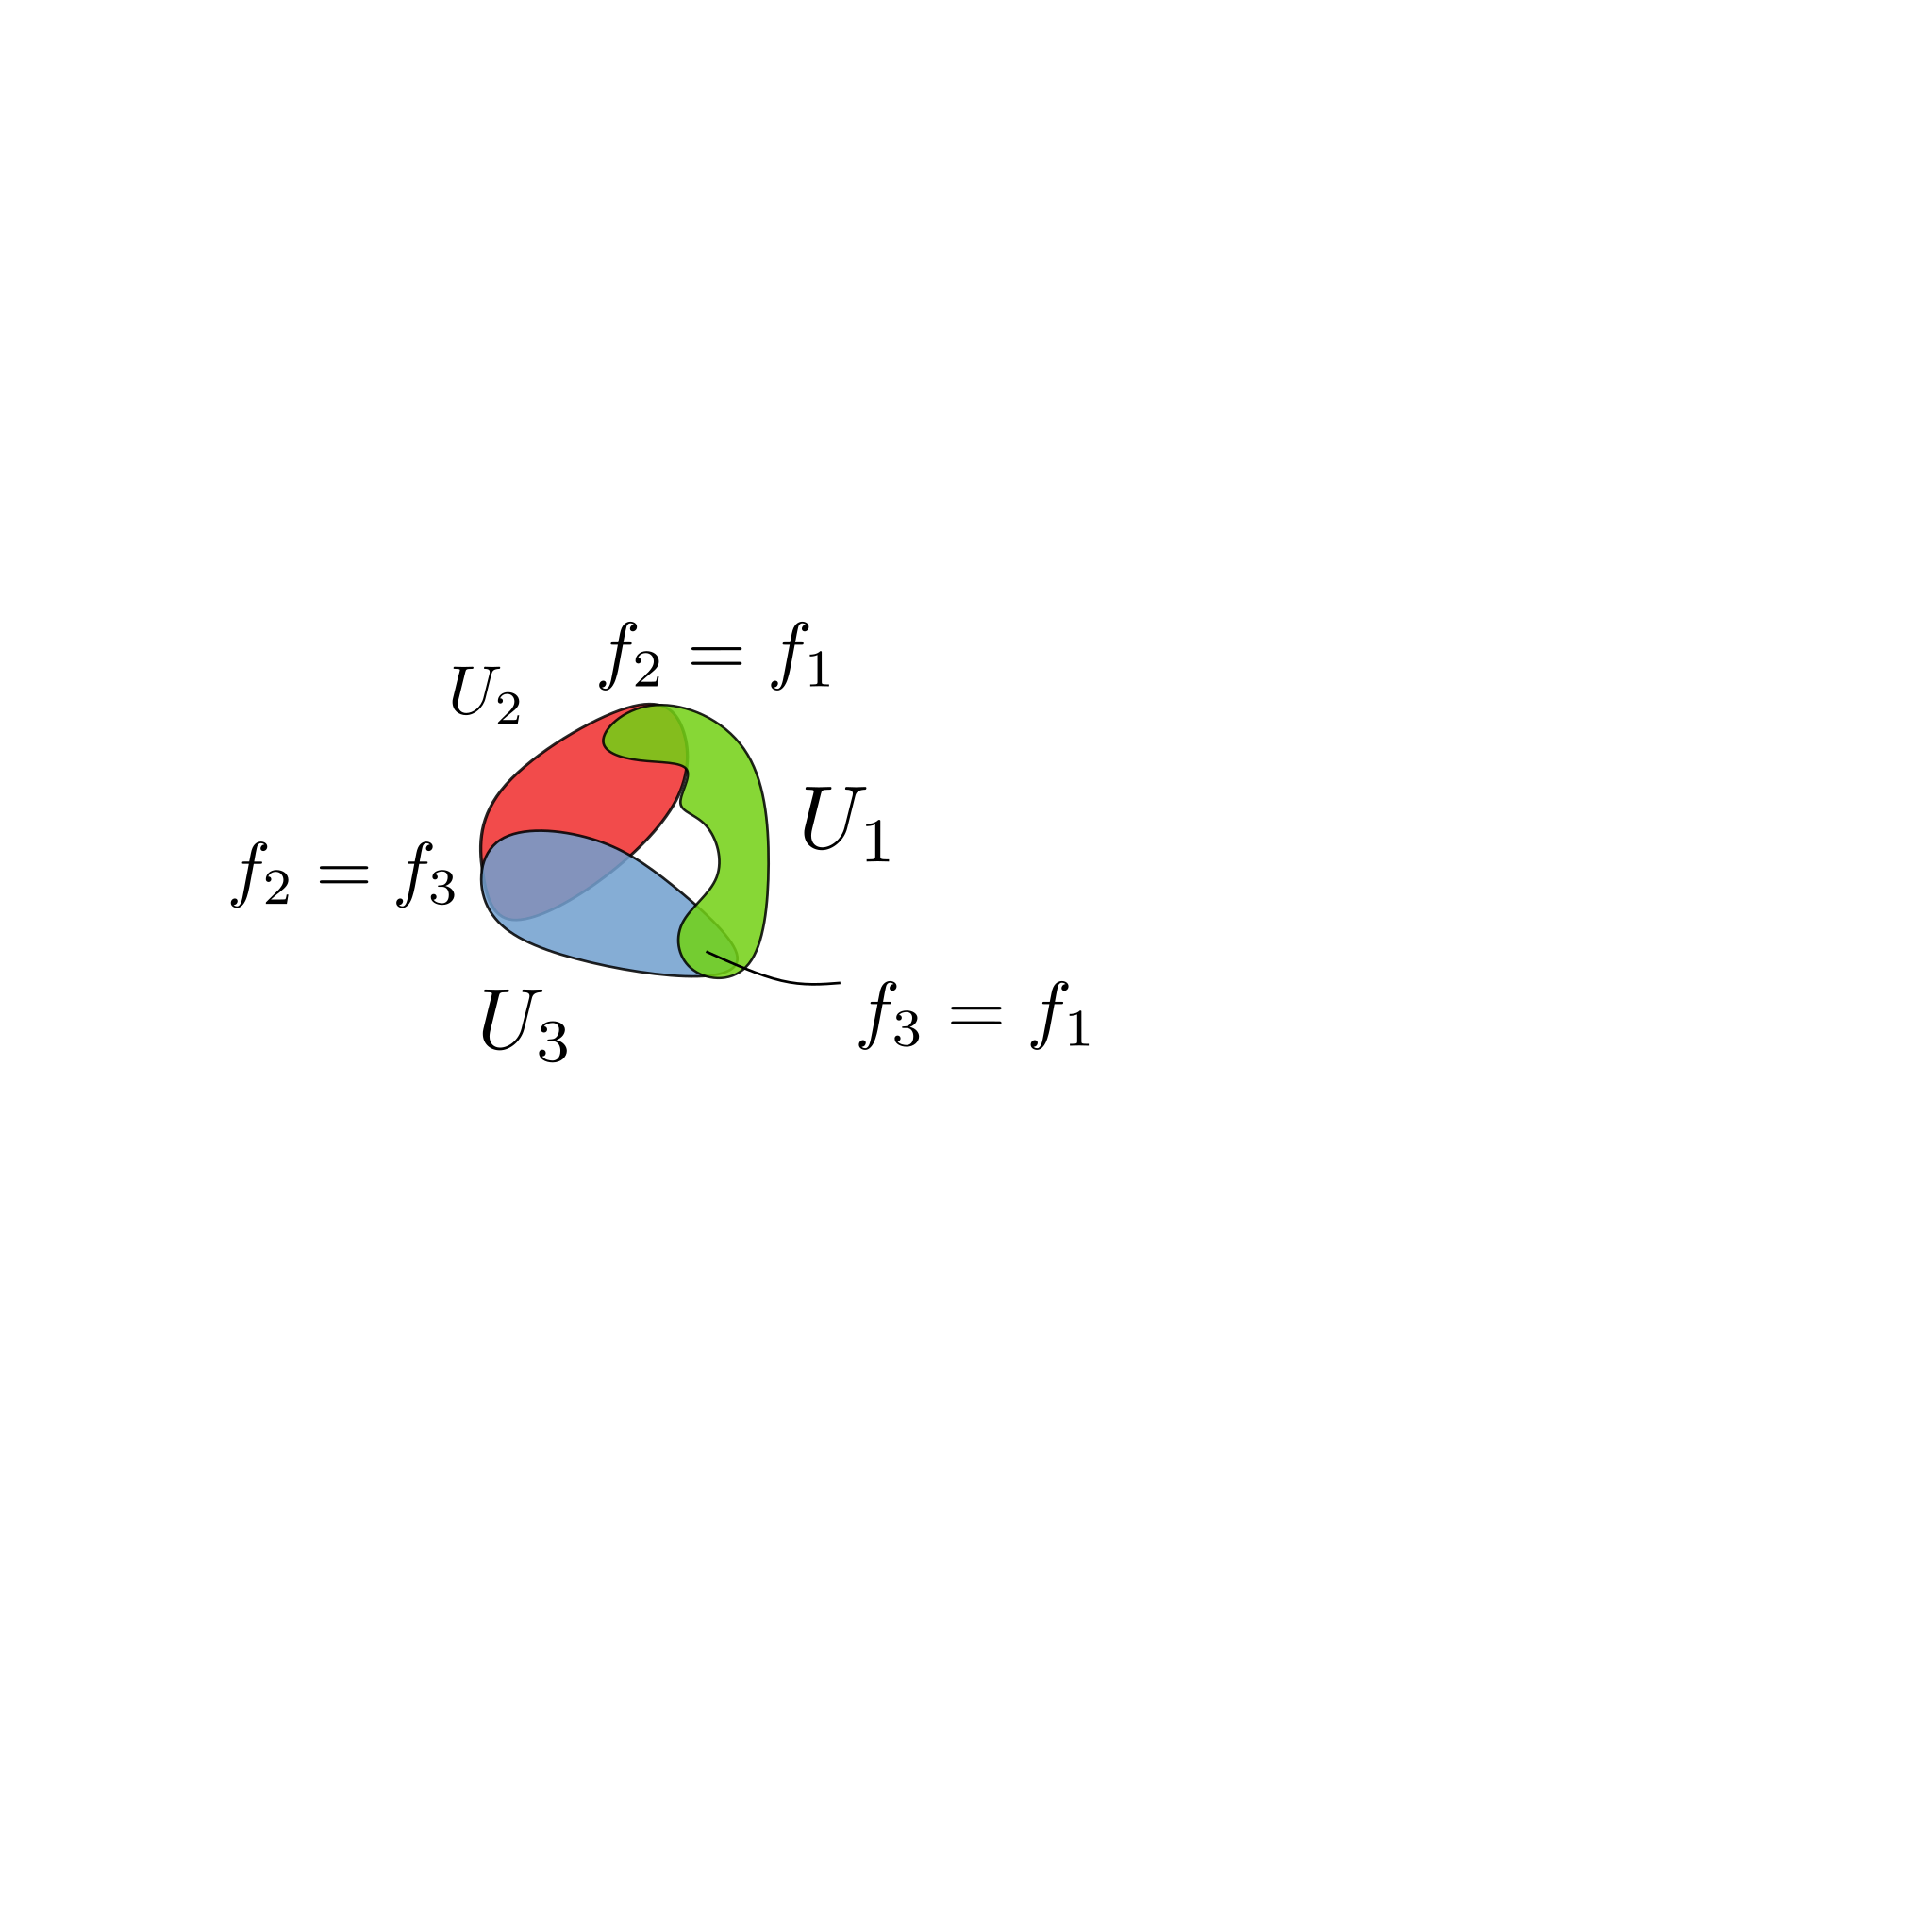
\includegraphics[width=.3\textwidth]{fig13-1}
        \caption{Tracimy jednoznaczność funkcji ale chyba worth it}
    \end{figure}
\end{przyklad}
\subsection{Klasyfikacja}
    Niech $f(z)$ - holomorficzna na pierścieniu $R(z_0, 0, r_1)$, ($f(z)$ może nawet nie być określona w $z_0$).\\
    Wiemy, że (działa wzór Laurenta):
    \[
        f(z) = \sum\limits_{n = -\infty}^{+\infty}a_n(z-z_0)^n
    .\]
Wyróżniamy trzy przypadki:
    \begin{enumerate}
        \item ($\Delta$) $a_n = 0$, $n < 0$:
            \[
                f(z) = \sum_{n = 0}^\infty a_n(z-z_0)^n = a_0 + a_1(z-z_0) + a_2(z-z_0)^2 + \dots
            \]
            Oznacza to, że przyjmując $f(z_0) = a_0$ otrzymamy funkcję holomorficzną na $K(r_0, r)$.
        \item ($\Delta\Delta$) $\underset{k<0}{\exists}\quad a_n = 0$, $n < k$
            \[
                f(z) = \sum_{n = 0}^\infty a_n(z-z_0)^n + \frac{a_{-1}}{(z-z_0)} + \frac{a_{-2}}{(z-z_0)} + \dots + \frac{a_{-k}}{(z-z_0)}
            \]
            O punkcie $z_0$ mówimy, że jest punktem osobliwym, izolowanym rzędu $|k|$. (albo, że jest biegunem rzędu $|k|$, np. $\frac{\cos(z)}{z}$ ma w $z_0 = 0$ biegun rzędu pierwszego).
        \item ($\Delta\Delta\Delta$)
            \[
                \underset{k < 0}{\forall}\quad \underset{n < k}{\exists}\quad a_n \neq 0
            \]
            \[
                f(z) = \sum_{n = 0}^\infty a_n(z-z_0)^n + \frac{a_{-1}}{(z-z_0)} + \frac{a_{-2}}{(z-z_0)^2} + \dots
            \]
            O punkcie $z_0$ powiemy, że jest punktem osobliwym (izolowanym) (albo, że $f(z)$ ma w $z = z_0$ osobliwość istotną).
    \end{enumerate}
\begin{przyklad}($\Delta$)\\
    \[
        f(z) = \frac{\sin(z)}{z}
    \]
    \[
        f(z) = \sum_{n = 0}^\infty (-1)^n \frac{z^n}{(2n+1)!} = 1 - \frac{x^2}{3!} + \frac{x^4}{5!} - \dots
    \]
    jeżeli przyjmiemy, że $f(0) = 1$, to jest
    \[
        f(z) = \begin{cases}\frac{\sin(z)}{z} & z \neq 0\\ 1 & z = 0\end{cases}
    \]
\end{przyklad}
\begin{przyklad}
    ($\Delta\Delta$)\\
    \[
        f(z) = \frac{\cos(z)}{z} = \sum_{n = 0}^\infty (-1)^n \frac{(z)^{2n - 1}}{(2n)!} = \underbrace{\frac{1}{z}}_{a_{-1}} - \frac{z}{2!} + \frac{z^3}{4!} + \dots
    \]
\end{przyklad}
\begin{przyklad}
    ($\Delta\Delta\Delta$)\\
    \[
        f(z) = \sum_{n = 0}^\infty \left(\frac{1}{z}\right)^n \cdot \frac{1}{n!}
    \]
\end{przyklad}
\begin{definicja}
    Liczbę $a_{-1}$ z rozwinięcia funkcji $f(z)$ w szerege Laurenta w pierścieniu $R(z_0, 0, r)$ nazywamy \textbf{residuum} funkcji $f(z)$ w $z_0$ i oznaczamy
    \[
        a_{-1} \equiv Res\{f(z)\} = \frac{1}{2\pi i} \int\limits_{\substack{K(z_0,r),\\ 0<r<r_1}} f(\xi)d\xi
    \]
\end{definicja}
\textbf{Uwaga: } mówimy (na razie) o osobliwościach izolowanych
\begin{przyklad}
    \[
        f(z) = \frac{1}{\sin\left(\frac{\pi}{z}\right)}
    .\]
Zauważmy, że $\sin\left(\frac{\pi}{z}\right) = 0 \iff z_n = \frac{1}{n}$, więc
    \[
        \lim\limits_{z\to 0}|f(z)| \to \infty,
    \]
    Więc $z_0 = 0$ nie jest osobliwością izolowaną, bo
    \[
        \underset{r > 0}{\forall}\quad\underset{n}{\exists}\quad z = \frac{1}{n}\in K(0,r).
    \]
\end{przyklad}
\begin{figure}[h]
    \centering
    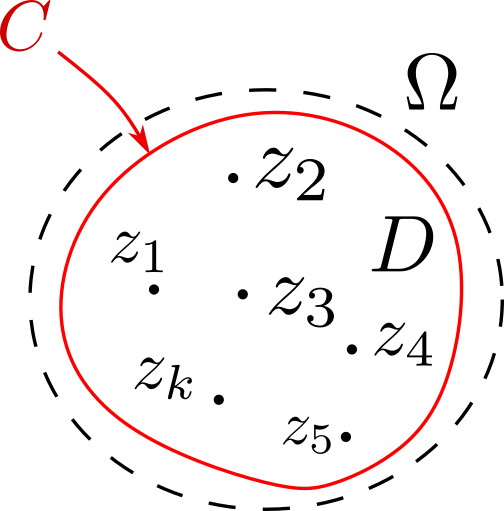
\includegraphics[width=.3\textwidth]{fig13-2}
\end{figure}
\begin{tw}
Niech $\Omega$ - otwarty, $D\subset \Omega$, $z_1,\dots,z_k\subset D,\quad z_i\cap \partial D = \{\phi\},\quad i = 1,\dots,k$, $f$ - holomorficzna na $\Omega - \{z_1,\dots,z_k\}$ i $z_i$ - bieguny funkcji $f$.\\
Wówczas
    \[
        \int\limits_{\partial D} f(z)dz = 2 \pi i \sum_{n=0}^k Res_{z = z_n}\{f(z)\}
    \]
\end{tw}
\begin{proof}
Rozważmy zbiór $P$ taki, jak na rys 13-3.
    Zauważmy, że $f(z)$ jest na $P$ holomorficzna. to znaczy, że
    \[
        \int\limits_{\partial P}f(z) dz = 0 = \int\limits{\partial D}f(z)dz + \sum_{n=1}^k \left[\quad\int\limits_{\partial K(z_n, r_n)}f(z) dz\right],
    \]
    czyli
    \[
        \int\limits_{\partial D} f(z) dz = 2 \pi i\sum_{n=1}^k Res_{z = z_k} f(z)
    .\]
\end{proof}
\textbf{Pytanie:} czy umiemy znaleźć współczynnik $a_{-1}$ bez roz funkcji $f$ w szereg Laurenta?\\
\textbf{Odpowiedź:} Jeżeli $f$ ma w $z_0$ biegun rzędu $n$, to znaczy, że
\[
    f(z) = \sum_{n=0}^\infty a_n(z-z_0)^n + \frac{a_{-1}}{(z-z_0)} + \dots
\]
\[
    Res_{z = z_k}f(z) = \lim\limits_{z\to z_k} \frac{1}{(n+1)!} \frac{d^{n-1}}{dz}\left((z-z_0)^nf(z)\right)
\]
\begin{przyklad}
    Policzyć całkę
    \[
        J = \int\limits_0^{2\pi} \frac{dx}{(1-2a\cos(x)+a^2)}
    \]
    Zauważmy, że
    \[
        1 - 2a \cos(x) + a^2 = 1 - 2a\left( \frac{e^{ix} + e^{-ix}}{2}\right) + a^2 \overset{?}{=} \frac{1}{z} (z-a)(1-az)
    \]
\end{przyklad}
\end{document}
